% Sablon pentru realizarea lucrarii de licenta, conform cu recomandarile
% din ghidul de redactare:
% - https://fmi.unibuc.ro/finalizare-studii/

% Multumiri lui Gabriel Majeri, acest sablon a fost creat pe baza
% codului sursa a lucrarii sale de licenta. 
% Codul sursa: https://github.com/GabrielMajeri/bachelors-thesis
% Website: https://www.gabrielmajeri.ro/
%
% Acest sablon este licentiat sub Creative Commons Attribution 4.0 International License.
% modificat 8 noiembrie 2024

\documentclass[12pt, a4paper]{report}

% Suport pentru diacritice și alte simboluri
\usepackage{fontspec}

% Font Times New Roman (bold/italic complet sub XeLaTeX)
\setmainfont{Times New Roman}
% Font monospațiat cu acoperire pentru diacriticele românești (cod inline + casete)
\setmonofont[Scale=0.92]{PT Mono}

% Evidențierea (\emph) se redă drept (fără cursive), ca în varianta anterioară
\renewcommand{\emph}[1]{\textup{#1}}

% Titluri de capitol/secțiune fără bold (ca înainte de fixarea fontului)
\usepackage{titlesec}
\titleformat{\chapter}[display]
  {\normalfont\huge}{\chaptertitlename\ \thechapter}{20pt}{\Huge}
\titlespacing*{\chapter}{0pt}{50pt}{40pt}
\titleformat*{\section}{\normalfont\Large}
\titleformat*{\subsection}{\normalfont\large}

% Suport pentru mai multe limbi
\usepackage{polyglossia}

% Setează limba textului la română
\setdefaultlanguage{romanian}
% Am nevoie de engleză pentru rezumat
\setotherlanguages{english}

% Indentează și primul paragraf al fiecărei noi secțiuni
\SetLanguageKeys{romanian}{indentfirst=true}

% Suport pentru diferite stiluri de ghilimele
\usepackage{csquotes}

\DeclareQuoteStyle{romanian}
  {\quotedblbase}
  {\textquotedblright}
  {\guillemotleft}
  {\guillemotright}

% Utilizează biblatex pentru referințe bibliografice
\usepackage[
    maxbibnames=50,
    sorting=nty
]{biblatex}

\addbibresource{bibliography.bib}
\setlength{\bibitemsep}{2pt}  % spațiere compactă între referințe

% Setează spațiere inter-linie (doublespacing din LaTeX este echivalentul setarii 1.5 in Microsoft Word)
\usepackage{setspace}
\doublespacing

% Modificarea geometriei paginii (cu margini de 2,5 cm) 
\usepackage[margin=2.5cm]{geometry}

% Include funcțiile de grafică
\usepackage{graphicx}
% Încarcă imaginile din directorul `images`
\graphicspath{{./images/}}

% Listări de cod
\usepackage{xcolor}
\usepackage{listings}
\definecolor{codebg}{rgb}{0.965,0.965,0.965}
\definecolor{codeframe}{rgb}{0.78,0.78,0.78}
\lstset{
  basicstyle=\ttfamily\small,
  breaklines=true,
  breakindent=0pt,
  frame=single,
  rulecolor=\color{codeframe},
  backgroundcolor=\color{codebg},
  framesep=8pt,
  framexleftmargin=8pt,
  xleftmargin=10pt,
  xrightmargin=6pt,
  aboveskip=1.2em,
  belowskip=1.2em,
  columns=fullflexible,
  keepspaces=true,
}

% Linii de tabel profesionale (\toprule, \midrule, \bottomrule)
\usepackage{booktabs}

% Diagrame (pipeline-ul sistemului)
\usepackage{tikz}
\usetikzlibrary{arrows.meta, positioning, fit, backgrounds, shapes.geometric}
\usepackage{forest}
\usepackage{float}

% Linkuri interactive în PDF
\usepackage[
    colorlinks,
    linkcolor={black},
    menucolor={black},
    citecolor={black},
    urlcolor={blue}
]{hyperref}

% Simboluri matematice codificate Unicode
\usepackage[warnings-off={mathtools-colon,mathtools-overbracket}]{unicode-math}

% Comenzi matematice
\usepackage{amsmath}
\usepackage{mathtools}

% Formule matematice
\newcommand{\bigO}[1]{\symcal{O}\left(#1\right)}
\DeclarePairedDelimiter\abs{\lvert}{\rvert}

% Suport pentru rezumat în două limbi
% Bazat pe https://tex.stackexchange.com/a/70818
\newenvironment{abstractpage}
  {\cleardoublepage\vspace*{\fill}\thispagestyle{empty}}
  {\vfill\cleardoublepage}
\renewenvironment{abstract}[1]
  {\bigskip\selectlanguage{#1}%
   \begin{center}\bfseries\abstractname\end{center}}
  {\par\bigskip}

% Suport pentru anexe
\usepackage{appendix}

% Stiluri diferite de headere și footere
\usepackage{fancyhdr}

% Metadate
\title{Asistent conversațional pentru proceduri administrative din România folosind RAG și local LLMs}
\author{Cosmin-Ștefan Glod}

% Generează variabilele cu @
\makeatletter

\begin{document}

% Front matter
\cleardoublepage
\let\ps@plain

% Pagina de titlu
\begin{titlepage}

% Redu marginile
\newgeometry{left=2cm,right=2cm,bottom=1cm}

\begin{figure}[!htb]
    \centering
    \begin{minipage}{0.2\textwidth}
        
\includegraphics[width=\linewidth]{logo-ub.png}
    \end{minipage}
    \begin{minipage}{0.5\textwidth}
        \large
        \vspace{0.2cm}
        \begin{center}
            \textbf{UNIVERSITATEA DIN BUCUREȘTI}
        \end{center}
        \vspace{0.3cm}
        \begin{center}
            \textbf{
                FACULTATEA DE \\
                MATEMATICĂ ȘI INFORMATICĂ
            }
        \end{center}
    \end{minipage}
    \begin{minipage}{0.2\textwidth}
        
\includegraphics[width=\linewidth]{logo-fmi.png}
    \end{minipage}
\end{figure}

\begin{center}
\textbf{SPECIALIZAREA INFORMATICĂ}
\end{center}

\vspace{0.5cm}

\begin{center}
\Large \textbf{Lucrare de licență}
\end{center}

\begin{center}
\LARGE \textbf{\@title}
\end{center}

\vspace{1.5cm}

\begin{center}
\large \textbf{Absolvent \\ \@author}
\end{center}

\vspace{0.25cm}

\begin{center}
\large \textbf{Coordonator științific \\ Prof. dr. Alin Ștefănescu}
\end{center}

\vspace{1.5cm}

\begin{center}
\Large \textbf{București, iunie 2026}
\end{center}
\end{titlepage}
\restoregeometry
\newgeometry{
    margin=2.5cm
}

\fancypagestyle{main}{
  \fancyhf{}
  \renewcommand\headrulewidth{0pt}
  \fancyhead[C]{}
  \fancyfoot[C]{\thepage}
}

\addtocounter{page}{1}

% Rezumatul
\begin{abstractpage}
\begin{singlespace}

\begin{abstract}{romanian}
Această lucrare prezintă un asistent conversațional destinat cetățenilor români, care răspunde la întrebări despre proceduri administrative (înregistrarea nașterii, încheierea căsătoriei și închirierea unei locuințe), pe baza datelor structurate publicate de proiectul Code for Romania pe \emph{cezicelegea.ro}. Sistemul folosește o arhitectură RAG (Retrieval-Augmented Generation) construită deasupra unui model lingvistic mare (LLM) cuantizat, executat local pe hardware de larg consum, fără apeluri către servicii externe. Spre deosebire de lucrările existente în domeniu, contribuția centrală este un strat de verificare a ieșirii: răspunsul modelului este forțat să se conformeze unei scheme tipizate, iar un set de reguli verifică, după generare, prezența și validitatea citațiilor și faptul că documentele menționate apar efectiv în surse, abordând astfel categoria de erori nesemnalate identificate ca lucrare viitoare în Gheorghe et al. (2026). Sunt prezentate arhitectura sistemului, alegerile de implementare și un cadru de evaluare a calității regăsirii, a fidelității răspunsurilor și a costului computațional, comparând niveluri de cuantizare și scări de model.
\end{abstract}

\begin{abstract}{english}
This thesis presents a conversational assistant for Romanian citizens that answers questions about administrative procedures (birth, marriage, housing), grounded in the structured data published by the Code for Romania project at \emph{cezicelegea.ro}. The system is built on a Retrieval-Augmented Generation (RAG) architecture on top of a quantized Large Language Model (LLM) running locally on commodity hardware, with no calls to external services. The central contribution, beyond data and domain choices, is an \emph{output-verification} layer: the model's response is constrained to a typed schema, and a set of rules check, after generation, the presence and validity of citations and that any mentioned documents actually appear in the sources, addressing the class of unflagged errors named as future work by Gheorghe et al. (2026). The thesis describes the system architecture, implementation decisions, and an evaluation framework covering retrieval quality, answer faithfulness, and computational cost across quantization levels and model scale.
\end{abstract}

\end{singlespace}
\end{abstractpage}


\tableofcontents

% Main matter
\cleardoublepage
\pagestyle{main}
\let\ps@plain\ps@main

\chapter{Introducere}

\section{Motivație și problemă}

Digitalizarea administrației publice este o prioritate europeană, urmărită în România prin platforme precum SPV-ul ANAF, Ghișeul.ro sau RO e-Factura. Beneficiul direct pentru cetățean rămâne însă limitat. Proceduri obișnuite, cum sunt înregistrarea unei nașteri, încheierea unei căsătorii sau închirierea unei locuințe, presupun interacțiuni cu mai multe instituții, reglementări care se modifică în timp și formulare specializate, fără o sursă unică de informare. Proiectul \emph{cezicelegea.ro} (Code for Romania) structurează informația pe \emph{evenimente de viață}, însă rămâne un site informativ. Cetățeanul identifică singur ramura din arborele decizional și completează formularele de la zero.

Asistenții conversaționali bazați pe modele lingvistice mari și pe RAG (Retrieval-Augmented Generation) pot transforma un astfel de corpus într-un dialog cu răspunsuri ancorate în surse. În sectorul public există însă două constrângeri importante: confidențialitatea, întrucât datele cetățeanului nu pot părăsi dispozitivul, și \emph{fidelitatea}, întrucât un răspuns plauzibil, dar nesusținut de surse, induce cetățeanul în eroare. Lucrarea abordează astfel întrebarea: \emph{cum poate fi construit un asistent pentru proceduri administrative românești care oferă răspunsuri verificabile și rulează integral pe hardware de larg consum, fără apeluri externe?}

\section{Obiective și contribuții}

Lucrarea își propune să construiască și să evalueze un pipeline RAG complet, executabil integral local, pentru trei evenimente de viață (naștere, căsătorie, locuire), care să ofere răspunsuri verificabile, ancorate în sursele oficiale. Elementul central urmărit este un strat de verificare a ieșirii care vizează exact categoria de erori nesemnalate indicată drept lucrare viitoare în Gheorghe et al.\ (2026) \cite{gheorghe2026robust}. În acest scop, lucrarea aduce următoarele contribuții:

\begin{itemize}
    \item \textbf{Strat de verificare a ieșirii}: generarea este constrânsă la o schemă JSON tipizată, iar un set de reguli verifică, după generare, prezența și validitatea citațiilor și faptul că documentele menționate apar în surse.
    \item \textbf{Cadru de evaluare reproductibil} al sistemului: pe un set de aur de întrebări, sunt măsurate calitatea regăsirii, fidelitatea răspunsurilor și costul computațional, comparând niveluri de cuantizare, scări de model și un model dintr-o altă familie, specializat pe limba română.
    \item \textbf{Pre-completarea formularelor} printr-un motor condus de specificații, care acoperă un catalog de formulare administrative și extrage automat câmpurile dintr-o conversație în limbaj natural.
    \item \textbf{Arhitectură integral locală}, pe hardware de larg consum, motivată de constrângerile de confidențialitate din sectorul public.
\end{itemize}

Față de lucrările grupului de cercetare (Gheorghe et al.\ \cite{gheorghe2026robust}; Paduraru et al.\ \cite{paduraru2026guardrail}), care propun arhitecturi multi-agent și injecție de erori, contribuția distinctă a acestei lucrări este implementarea și evaluarea concretă a stratului de verificare a ieșirii, pe o sursă de date și evenimente disjuncte, cu execuție locală.

\chapter{Preliminarii}

\section{RAG (Retrieval-Augmented Generation)}

Un model lingvistic mare generează răspunsuri pe baza tiparelor învățate la antrenare, fixate în parametrii săi. Pentru informație absentă din datele de antrenare, modelul fie semnalează că nu o deține, fie generează un răspuns plauzibil, dar nesusținut, cu aceeași certitudine ca unul corect (\emph{halucinație} \cite{ji2023hallucination}). În domenii cu miză ridicată (juridic, medical, administrativ), un astfel de răspuns fals poate fi mai dăunător decât recunoașterea lipsei de informație.

\emph{RAG} (Retrieval-Augmented Generation) \cite{lewis2020retrieval} atenuează acest risc schimbând sursa răspunsului: modelul nu mai generează din cunoașterea parametrică, ci pe baza unor documente regăsite în prealabil. Procesul cuprinde două etape: \emph{regăsirea}, în care sistemul selectează automat fragmentele cele mai relevante pentru întrebare, și \emph{generarea}, în care răspunsul este compus pe baza acelor fragmente, oferite modelului ca \emph{context}. Răspunsul devine astfel ancorat în surse, poate fi însoțit de citații verificabile, iar riscul de halucinație scade \cite{gao2023retrieval}. În plus, RAG separă cunoașterea (documentele) de capacitatea de a genera text, astfel încât actualizarea informației nu necesită reantrenarea modelului.

\section{Reprezentări vectoriale și regăsire}

Abordarea clasică de regăsire este cea \emph{lexicală}, în care un fragment este relevant dacă împărtășește cuvinte cu întrebarea, ponderate după frecvență (familia \emph{BM25} \cite{robertson2009bm25}). Metoda este rapidă, dar compară forme de cuvinte, nu sensuri: o întrebare despre „acte necesare" nu se potrivește cu un text despre „documente obligatorii", deși înțelesul este același (\emph{nepotrivire de vocabular}). În limba română problema se accentuează din cauza flexiunii bogate, care multiplică formele de suprafață ale aceluiași cuvânt.

Soluția este compararea sensului. Pornind de la observația că două cuvinte cu contexte asemănătoare au înțelesuri asemănătoare, cuvintele au fost reprezentate prin vectori \emph{denși} (de exemplu \emph{word2vec} \cite{mikolov2013efficient}); modelele neuronale ulterioare au extins ideea la fraze și fragmente întregi, transformând un text într-un singur vector, numit \emph{embedding}. Regăsirea devine astfel \emph{semantică} (\emph{dense retrieval} \cite{karpukhin2020dense}): întrebarea și fragmentele sunt transformate în embeddings de același model (de exemplu multilingvul \emph{BGE-M3} \cite{chen2024bgem3}), iar relevanța este dată de apropierea vectorilor, măsurată prin \emph{similaritate cosinus}. Pentru a evita compararea cu toți vectorii, regăsirea folosește o indexare aproximativă a vecinilor, de exemplu \emph{HNSW} \cite{malkov2020hnsw}, oferită de baze de date vectoriale precum \emph{Chroma} \cite{chroma}.

\section{Modele lingvistice locale}
\label{sec:cuantizare}

Confidențialitatea datelor impune adesea ca modelul să ruleze local, fără transmiterea acestora către servicii externe; principala constrângere devine atunci memoria, determinată de numărul de \emph{biți} alocați fiecărui parametru. Implicit, un parametru ocupă 32 de biți (\texttt{FP32}), deci un model de 3 miliarde de parametri necesită $\sim$12~GB, prea mult pentru un calculator obișnuit. \emph{Cuantizarea} \cite{frantar2023gptq} reduce numărul de biți per parametru: modelul ocupă mai puțin și se evaluează mai rapid, în schimbul preciziei. Nivelurile uzuale pentru un model 3B sunt:

\begin{itemize}
    \item \texttt{FP16} (16 biți): aproximativ jumătate din memorie ($\sim$6~GB), cu pierdere de precizie practic neglijabilă;
    \item \texttt{Q8} (8 biți întregi): $\sim$3~GB, cu degradare redusă a calității;
    \item \texttt{Q4} (4 biți întregi): $\sim$2~GB, cea mai agresivă comprimare uzuală, cu risc real de degradare a raționamentului.
\end{itemize}

Schemele \emph{k-quants} din \texttt{llama.cpp} (sufixul \texttt{\_K\_M}) nu comprimă uniform, ci păstrează la precizie mai mare parametrii importanți, obținând un compromis mai bun. Astfel de modele se rulează local prin \texttt{llama.cpp} (format \texttt{GGUF}) sau prin interfețe precum \emph{Ollama} \cite{ollama}. Pe lângă cuantizare, modelele locale se diferențiază prin \emph{scară} (numărul de parametri: modelele mai mari raționează mai fidel, dar cer mai multe resurse) și prin \emph{specializare lingvistică}: un model generalist multilingv (Qwen2.5 \cite{yang2024qwen25}) acoperă multe limbi, în timp ce unul antrenat special pe o limbă cu resurse reduse (RoLlama3 \cite{masala2024openllmro}) poate compensa subreprezentarea ei.

\section{Verificarea ieșirii}
\label{sec:contracte}

În contexte reglementate, generarea de text liber nu este suficientă: răspunsul trebuie să poată fi verificat. Gheorghe et al.\ (2026) \cite{gheorghe2026robust} arată empiric că aproximativ 63\% dintre erorile injectate la limitele serviciilor externe rămân \emph{nesemnalate} (modelul produce răspunsuri plauzibile pe date incomplete) și propun verificarea sistematică a ieșirii ca direcție de cercetare. Un strat de \emph{verificare a ieșirii} are două componente: o \emph{schemă structurată} (un format tipizat, de exemplu JSON, impus motorului de inferență, care elimină erorile de formă) și un \emph{set de reguli aplicate după generare}, care verifică proprietăți de conținut, precum existența și validitatea citațiilor și prezența în surse a documentelor menționate. La eșec, generarea poate fi reluată cu feedback explicit, iar la epuizarea încercărilor răspunsul devine un refuz controlat.

Verificarea externă se distinge de cea integrată în model (\emph{Self-RAG} \cite{asai2024selfrag}) și se înrudește cu \emph{guardrails} programabile (NeMo Guardrails \cite{rebedea2023nemo}) și cu cadre de evaluare a RAG (RAGAS \cite{es2024ragas}); spre deosebire de un model-judecător extern, regulile de verificare sunt deterministe, auditabile și rulează integral local.

\chapter{Sistemul propus}

\section{Vedere de ansamblu}

Sistemul implementează un pipeline RAG complet pentru cele trei evenimente de viață de pe \emph{cezicelegea.ro} \cite{cezicelegea} (naștere, căsătorie, locuire), rulând local după descărcarea inițială a modelelor. Se compune din șase module Python: \textbf{scraper}, \textbf{chunker} (segmentare cu breadcrumb), \textbf{index} (embedding + Chroma), \textbf{retriever}, \textbf{generator} (LLM cu constrângere de schemă) și \textbf{contracts} (reguli de verificare a ieșirii).

\begin{figure}[tb]
    \centering
    \resizebox{\textwidth}{!}{%
    \begin{tikzpicture}[
        font=\small,
        node distance=0.5cm and 0.7cm,
        box/.style={draw, rounded corners, align=center, minimum height=1cm,
            minimum width=1.9cm, fill=blue!8},
        data/.style={draw, align=center, minimum height=1cm,
            minimum width=1.7cm, fill=gray!12},
        arr/.style={-{Stealth[length=2mm]}, thick},
    ]
        % offline (indexing) row
        \node[data] (web) {cezicelegea.ro\\\scriptsize (HTML)};
        \node[box, right=of web] (scrap) {scraper};
        \node[box, right=of scrap] (chunk) {chunker\\\scriptsize breadcrumb};
        \node[box, right=of chunk] (emb1) {BGE-M3\\\scriptsize embedding};
        \node[data, right=of emb1] (chroma) {Chroma\\\scriptsize 147 vectori};
        \draw[arr] (web) -- (scrap);
        \draw[arr] (scrap) -- (chunk);
        \draw[arr] (chunk) -- (emb1);
        \draw[arr] (emb1) -- (chroma);

        % online (serving) row
        \node[data, below=1.6cm of web] (q) {Întrebare};
        \node[box, right=of q] (emb2) {BGE-M3\\\scriptsize embedding};
        \node[box, right=of emb2] (ret) {retriever\\\scriptsize top-$k$=4};
        \node[box, right=of ret] (gen) {generator\\\scriptsize Qwen2.5 + schemă};
        \node[box, right=of gen] (contr) {verificare\\\scriptsize R1-R7};
        \node[data, right=of contr] (out) {Răspuns +\\\scriptsize citații / PDF};
        \draw[arr] (q) -- (emb2);
        \draw[arr] (emb2) -- (ret);
        \draw[arr] (ret) -- (gen);
        \draw[arr] (gen) -- (contr);
        \draw[arr] (contr) -- (out);

        % index feeds retriever
        \draw[arr] (chroma) -- (ret);
        % retry loop
        \draw[arr] (contr) to[out=110, in=70] node[above, font=\scriptsize] {reîncercare dacă răspunsul e invalid} (gen);

        \begin{scope}[on background layer]
            \node[draw=gray!40, dashed, rounded corners, fit=(web)(chroma),
                label={[gray, font=\scriptsize]above:Offline: construirea indexului}] {};
            \node[draw=gray!40, dashed, rounded corners, fit=(q)(out),
                label={[gray, font=\scriptsize]below:Online: servirea unei întrebări}] {};
        \end{scope}
    \end{tikzpicture}}
    \caption{Arhitectura sistemului, cu faza offline de construire a indexului și faza online de servire a unei întrebări.}
    \label{fig:pipeline}
\end{figure}

\section{Date și segmentare}

Conținutul de pe \emph{cezicelegea.ro} este o aplicație de tip \emph{state machine} pe partea de client (Alpine.js): întreg arborele de decizie al fiecărui eveniment este prezent în HTML-ul static, dar vizibilitatea fiecărui nod este controlată în browser. Scraperul (\texttt{requests} + \texttt{BeautifulSoup} \cite{beautifulsoup}, fără motor de browser) parsează DOM-ul static și \emph{reconstruiește offline} arborele real: îl parcurge în pre-ordine (DFS) cu o stivă de context, luând conținutul nodului din titlurile \texttt{h2} și etichetele copiilor din \texttt{h3}-urile butoanelor de navigare. Deoarece etichetele sunt uneori prescurtate, potrivirea părinte-copil folosește o similaritate Jaccard pe cuvinte (prag $0.7$). Rezultă 107 secțiuni cu \emph{breadcrumb} complet (până la 8-9 niveluri), cu cele trei ramuri principale reconstruite corect.

\begin{figure}[H]
    \centering
    \begin{forest}
      for tree={
        font=\footnotesize, grow'=0,
        child anchor=west, parent anchor=south, anchor=west, calign=first,
        draw=gray!55, rounded corners, fill=blue!5, inner sep=2.5pt,
        edge={draw, gray!55},
        edge path={\noexpand\path[\forestoption{edge}]
          (!u.south west) +(6pt,0) |- (.child anchor)\forestoption{edge label};},
        before typesetting nodes={if n=1{insert before={[,phantom]}}{}},
        fit=band, before computing xy={l=16pt}, s sep=1.2mm,
      }
      [Nașterea, fill=blue!15
        [Certificatul medical constatator [\ldots]]
        [Certificatul de naștere
          [Sunt cetățean român
            [Nașterea a avut loc în România
              [Partenerul este cetățean român
                [Suntem soți]
                [Nu suntem căsătoriți
                  [Tatăl recunoaște copilul]
                  [Tatăl nu recunoaște copilul]
                ]
              ]
              [Partenerul este cetățean străin [\ldots]]
            ]
            [Nașterea a avut loc în străinătate [\ldots]]
          ]
          [Sunt cetățean străin [\ldots]]
        ]
        [Ajutor financiar
          [Stimulente pentru nou-născut]
          [Alocația de stat pentru copii [\ldots]]
          [\ldots]
        ]
      ]
    \end{forest}
    \caption{Fragment simplificat din arborele de decizie al evenimentului \emph{Nașterea}, reconstruit offline din DOM-ul static (subarborii marcați cu \ldots\ sunt omiși). Arborele real atinge 8-9 niveluri; fiecare frunză primește un breadcrumb complet, prefixat în textul indexat.}
    \label{fig:tree}
\end{figure}

Modulul \texttt{chunker} prefixează breadcrumb-ul în textul indexat, sub forma \texttt{[Nașterea > Certificatul de naștere > {\ldots} > Tatăl recunoaște copilul]} urmată de conținut (Figura~\ref{fig:tree}). Prefixul contribuie la embedding și distinge ramuri semantice apropiate (de exemplu, documente pentru cuplu căsătorit versus pentru un părinte necăsătorit), păstrând trasabilitatea sursei. Secțiunile mai mari de $\sim$3000 de caractere sunt împărțite greedy la limite de propoziție; indexul final conține 147 de fragmente.

\section{Regăsire și generare}

Embedding-urile sunt calculate cu \emph{BGE-M3} \cite{chen2024bgem3} (multilingv, 1024 de dimensiuni), normalizate L2 astfel încât similaritatea cosinus din \emph{Chroma} să se reducă la produs scalar. La interogare, baza returnează cele mai relevante $k = 4$ fragmente. Valoarea este un compromis (un $k$ prea mic ratează fragmentul cu răspunsul, iar unul prea mare diluează contextul și crește costul), iar la $k = 4$ regăsirea acoperă deja aproape integral fragmentele relevante (Capitolul~\ref{cap:evaluare}). Cele trei evenimente formează grupuri bine separate în spațiul de embedding, ceea ce explică recall-ul ridicat al regăsirii (Figura~\ref{fig:embeddings}).

\begin{figure}[H]
    \centering
    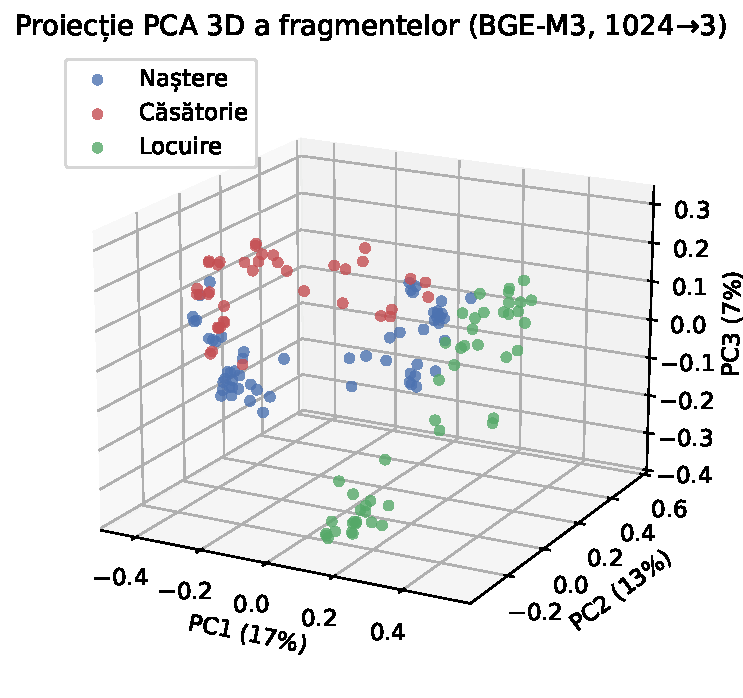
\includegraphics[width=0.62\textwidth]{fig_embeddings.pdf}
    \caption{Fragmentele celor trei evenimente, separate în spațiul de embedding.}
    \label{fig:embeddings}
\end{figure}

Generarea rulează \emph{integral local} prin Ollama (peste \texttt{llama.cpp}, format \texttt{GGUF}); configurația implicită este \emph{Qwen2.5-3B-Instruct} \cite{yang2024qwen25}, suficient de mică pentru hardware de larg consum. Apelul conține un prompt de sistem care impune limba română și ancorarea strictă în surse, un mesaj de utilizator cu sursele numerotate \texttt{[S1]} \ldots \texttt{[Sn]} și întrebarea, plus o schemă JSON derivată din clasa Pydantic \cite{pydantic} \texttt{AnswerSchema}, transmisă prin parametrul \texttt{format} pentru a forța conformitatea structurală.

Promptul de sistem (redat condensat mai jos) codifică regulile de comportament pe care stratul de verificare a ieșirii le controlează ulterior automat:

\begin{center}
\setlength{\fboxsep}{8pt}%
\fcolorbox{codeframe}{codebg}{%
\begin{minipage}{0.9\textwidth}
\ttfamily\small\raggedright
Ești un asistent care ajută cetățenii români să înțeleagă proceduri administrative (naștere, căsătorie, locuire). Respectă strict următoarele reguli:\\[3pt]
(1) Răspunde exclusiv în limba română.\\
(2) Bazează-te numai pe SURSELE furnizate; nu inventa documente, termene, instituții sau cifre.\\
(3) Indică sursele folosite prin indici (de exemplu, sursele 1 și 3 -> cited\_source\_indices=[1,3]).\\
(4) Dacă SURSELE nu conțin răspunsul, setează is\_refusal=true și răspunde: „Nu am suficiente informații în sursele disponibile pentru a răspunde."\\
(5) În documents\_mentioned trece doar numele reale de documente care apar explicit în SURSE.\\
(6) Formulează răspunsul concis și structurat.\\
(7) Setează form\_offer numai dacă utilizatorul își exprimă intenția de a completa un formular.
\end{minipage}}
\end{center}

Schema răspunsului are cinci câmpuri: \texttt{answer\_text}, \texttt{is\_refusal}, \texttt{cited\_source\_indices}, \texttt{documents\_mentioned} și \texttt{form\_offer}. Ultimele două sunt esențiale pentru regulile care împiedică inventarea de documente, respectiv pentru tranziția către pre-completarea formularelor.

\section{Stratul de verificare a ieșirii}

După obținerea răspunsului structurat, sistemul aplică reguli automate care verifică nu \emph{forma} (garantată de schemă), ci \emph{conținutul}: măsura în care răspunsul se sprijină pe surse. Fiecare regulă vizează un mod în care un răspuns poate părea corect, dar poate induce cetățeanul în eroare:

\begin{itemize}
    \item \textbf{R1: existența unui răspuns.} Verifică faptul că schema conține un text de răspuns nevid (câmpul \texttt{answer\_text}). \emph{Motivație:} prinde eșecurile complete de generare (răspuns gol, ieșire degenerată sau generare întreruptă), care altfel ar fi servite cetățeanului ca răspuns valid. Această regulă este totodată o precondiție pentru celelalte reguli, întrucât fără text nu există ce cita sau ancora.
    \item \textbf{R2: citarea afirmațiilor.} Un răspuns care nu este refuz trebuie să indice cel puțin o sursă. \emph{Motivație:} în lipsa citației, informația nu poate fi verificată, iar un fapt real nu poate fi distins de unul inventat.
    \item \textbf{R3: validitatea citațiilor.} Indicii citați trebuie să existe efectiv în lista de surse (între 1 și $n$). \emph{Motivație:} o trimitere la ,,sursa 7" atunci când există doar 4 surse reprezintă o citație inventată.
    \item \textbf{R4: ancorarea documentelor menționate.} Orice document numit în răspuns trebuie să se regăsească în textul sursei citate. \emph{Motivație:} este principala regulă care prinde documentele inventate, identificând situațiile în care modelul indică un act sau un formular ce nu există în procedură.
    \item \textbf{R5: refuzul nu menționează documente.} Atunci când modelul refuză să răspundă, nu are voie să enumere documente. \emph{Motivație:} un refuz însoțit de documente reprezintă o invenție mascată: pare prudent, dar introduce informație nesusținută.
    \item \textbf{R6: absența identificatorilor interni de formular.} Identificatorii tehnici (de exemplu \texttt{declaratie\_nume\_copil}) nu trebuie confundați cu nume reale de acte. \emph{Motivație:} se evită expunerea catalogului intern de formulare în răspunsul oferit cetățeanului.
\end{itemize}

Regulile R1-R6 constituie setul evaluat în Capitolul~\ref{cap:evaluare}. Ulterior a fost adăugată regula \textbf{R7}, care semnalează un \emph{refuz nejustificat}: modelul refuză, deși o sursă regăsită cu similaritate ridicată conține răspunsul. \emph{Motivație:} este singura regulă care vizează modul de eșec dominant, în care cetățeanul primește un refuz la o întrebare legitimă. Acest mod de eșec este invizibil pentru R1-R6, deoarece un refuz nu conține nici citații, nici documente care să poată fi verificate.

Limba de răspuns nu este verificată printr-o regulă separată, deoarece este deja impusă de promptul de sistem și a fost respectată de toate modelele evaluate. Regulile R1-R7 se concentrează pe modul de eșec relevant pentru fidelitate: ancorarea răspunsului în surse.

Atunci când o regulă nu este satisfăcută și mai există încercări disponibile, sistemul reapelează modelul cu un mesaj de feedback explicit. La epuizarea încercărilor (implicit una), răspunsul este marcat drept \emph{invalid}, iar interfața afișează un refuz controlat.

În testarea manuală s-au observat trei comportamente. Pentru întrebări clare, sistemul produce răspunsuri ancorate în surse. Pentru întrebări care combină mai multe evenimente, regăsirea este dominată de termenul cu pondere mai mare, iar modelul refuză în loc să fabrice. Pentru întrebări din afara domeniului, modelul tinde să genereze o procedură generică, pe care verificarea o identifică prin R2 sau R4.

\section{Pre-completarea formularelor și interfața}

Sistemul include un strat de pre-completare a formularelor, declanșat atunci când utilizatorul își exprimă intenția (prin câmpul \texttt{form\_offer} și un detector pe cuvinte-cheie). Stratul este \emph{condus de specificații}: fiecare formular este declarat o singură dată, ca listă de câmpuri tipizate, din care se derivă automat schema Pydantic, validatorul (CNP, serie și număr CI, dată ISO 8601, IBAN), randarea PDF (\texttt{fpdf2} \cite{fpdf2}) și extractorul; astfel, adăugarea unui formular nou se reduce la o descriere declarativă, fără cod suplimentar. Catalogul acoperă șapte formulare pe cele trei evenimente. Extragerea folosește o schemă JSON partiționată pe secțiuni (3-6 câmpuri), pentru a evita omiterea câmpurilor; la eșec, sistemul comută la un mod manual cu validare prin expresii regulate, garantând producerea unui PDF semnabil.

\begin{figure}[H]
    \centering
    \fbox{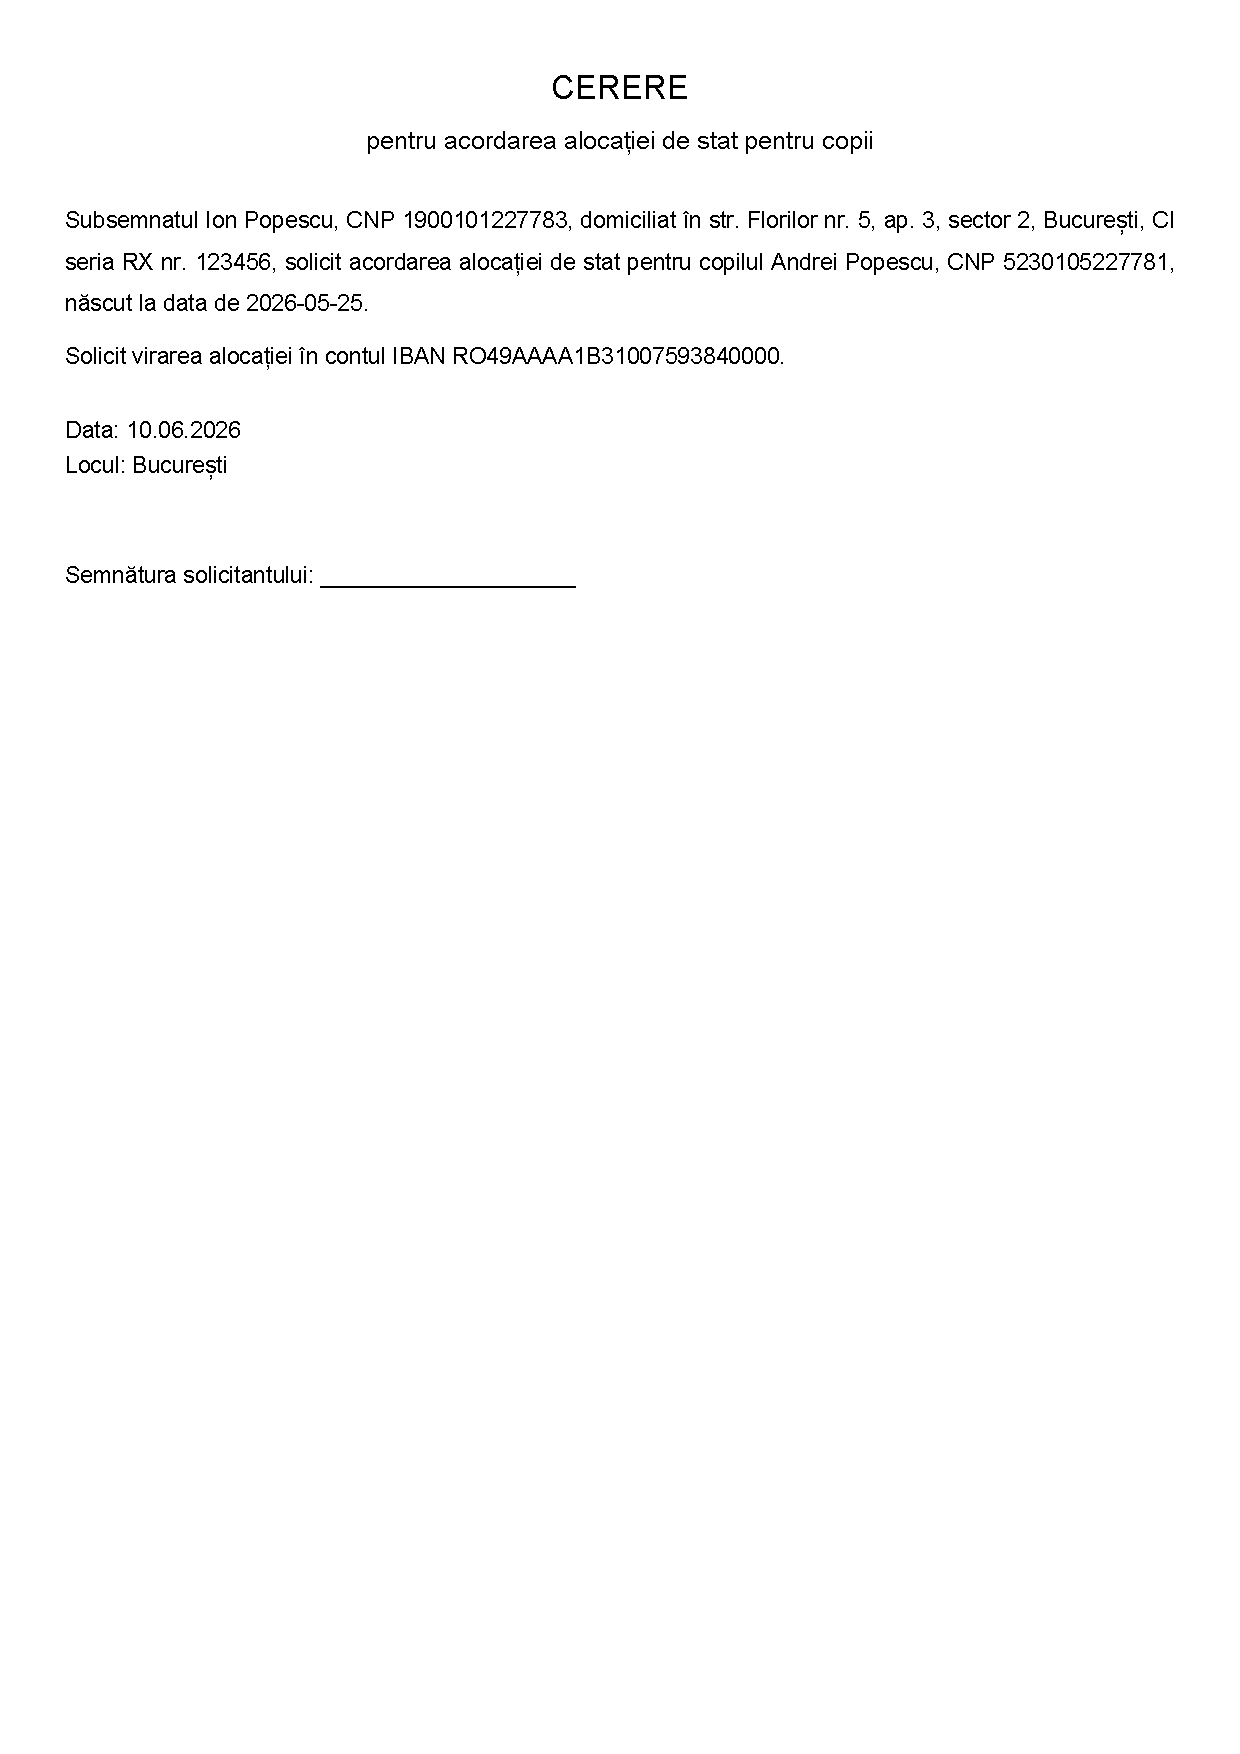
\includegraphics[width=0.75\textwidth, trim={1cm 18.5cm 1cm 0.8cm}, clip]{cerere_alocatie.pdf}}
    \caption{Antetul și corpul unui formular generat de stratul de pre-completare (cererea pentru alocația de stat), pornind de la datele extrase dintr-o conversație în limbaj natural.}
    \label{fig:sampleform}
\end{figure}

Interfața web (\emph{Streamlit} \cite{streamlit}) afișează conversația, sursele citate marcate distinct și butoanele de descărcare a formularelor, deschizând la nevoie blocul de pre-completare cu intrare generată de model sau introdusă manual (Figura~\ref{fig:interfata}). Interfața folosește aceeași infrastructură ca varianta în linie de comandă, ceea ce asigură un comportament unic, derivat dintr-o singură sursă de adevăr.

\begin{figure}[H]
    \centering
    \fbox{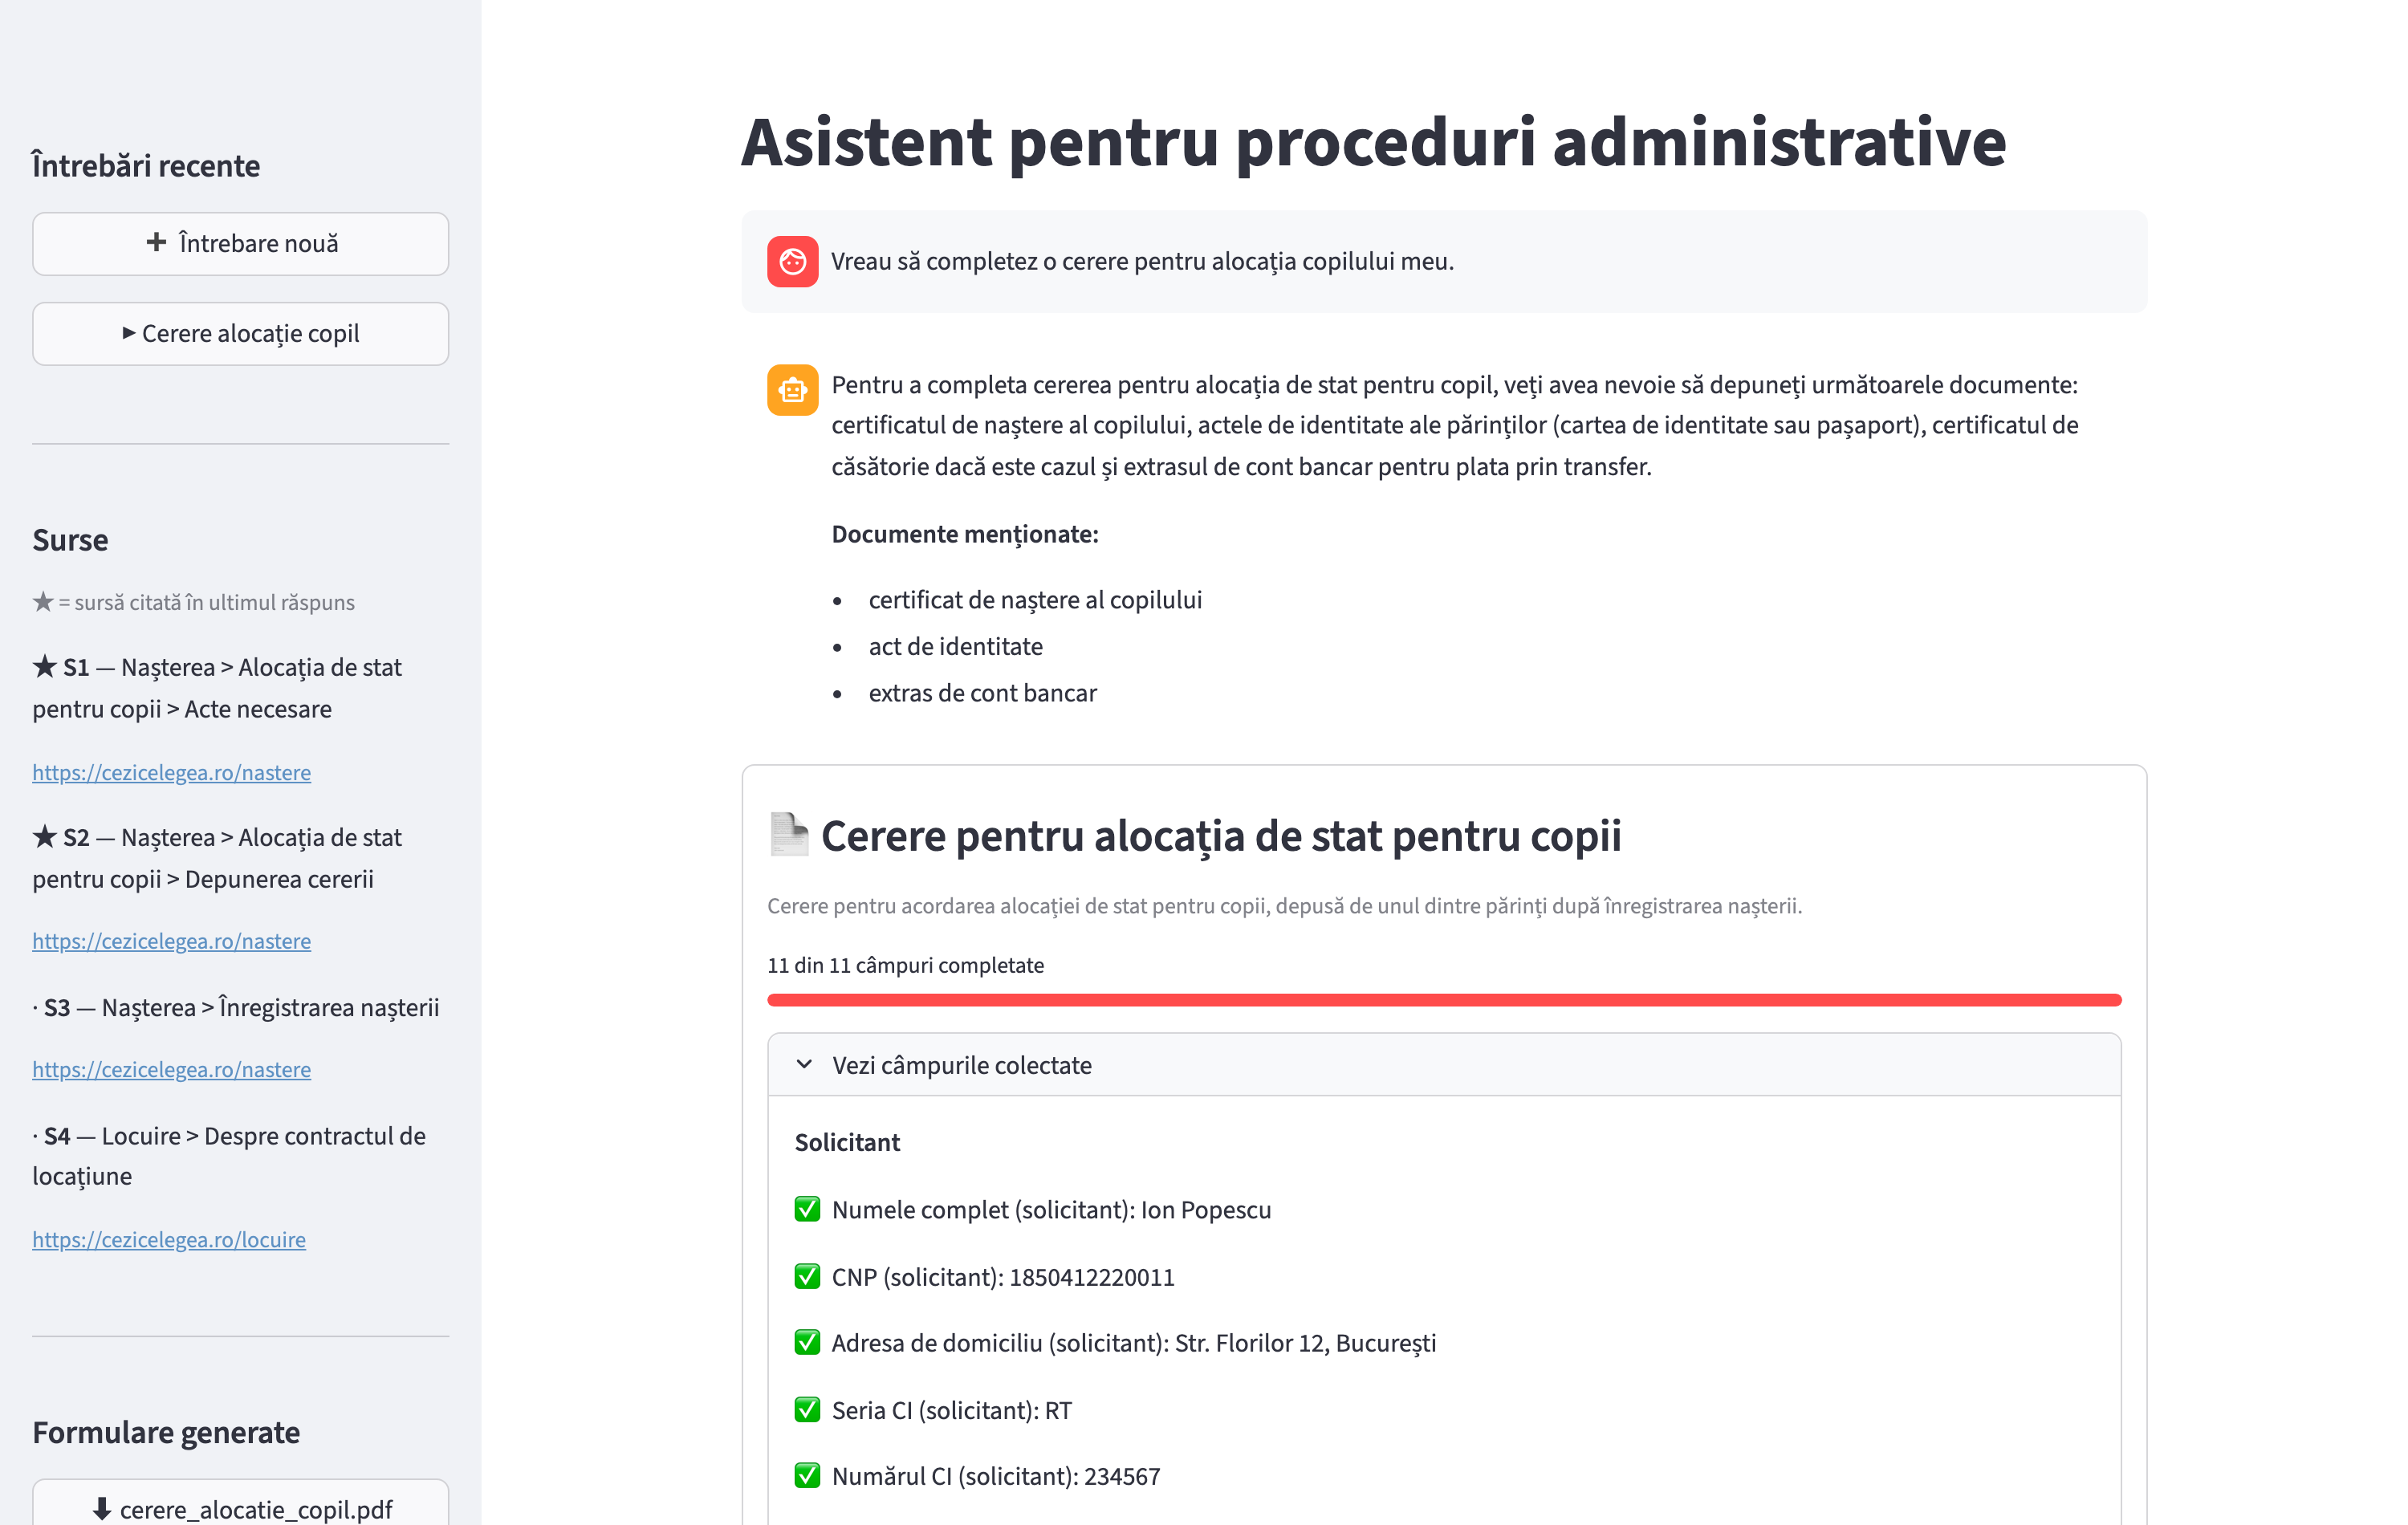
\includegraphics[width=0.75\textwidth]{interfata_completa.png}}
    \caption{Interfața web: în bara laterală, istoricul de întrebări și panoul \emph{Surse} (sursele citate marcate distinct); în centru, dialogul cu modelul și blocul de pre-completare a formularelor.}
    \label{fig:interfata}
\end{figure}

\chapter{Rezultate}
\label{cap:evaluare}

\section{Setup și metrici}

Sistemul este evaluat pe un set de aur de 98 de cazuri (35 naștere, 30 căsătorie, 33 locuire), dintre care 16 de tip \emph{refuz controlat} (în afara domeniului); proveniența și validarea sa sunt discutate în Secțiunea~\ref{sec:limitari}. Toate rulările folosesc aceiași parametri ($k=4$, o singură reîncercare, temperatura 0) și aceeași infrastructură (GPU 2$\times$Tesla T4). Comparația cantitativă principală este un \textbf{studiu comparativ} a șase configurații: modelul 3B la trei niveluri de cuantizare (FP16, Q8, Q4) și două scări mai mari la Q4 (7B și 14B), plus un model RO-specializat din altă familie (RoLlama3-8B), rulat prin pipeline-ul complet. Codul sursă, setul de aur și artefactele de evaluare sunt disponibile public la \url{https://github.com/cosmin-glod/Romanian-Legal-Document-Assistent}, pentru reproductibilitate.

Se calculează cinci metrici: \emph{refusal accuracy} (\texttt{is\_refusal} vs \texttt{should\_refuse}), \emph{breadcrumb recall@k}, \emph{lexical keyword recall} (potrivire exactă de sub-șir a cuvintelor-cheie așteptate), \emph{rată de validare} (cazuri care trec toate regulile R1-R6) și \emph{latency}. Recall-ul de breadcrumb și cel de cuvinte-cheie sunt \emph{proxy-uri}: al doilea este o limită inferioară a fidelității (nu recunoaște sinonime), triangulată mai jos printr-un eșantion evaluat manual.

\section{Rezultate principale}

Tabelul~\ref{tab:sweep} sintetizează rezultatele celor șase configurații: modelul 3B la trei niveluri de cuantizare (FP16, Q8, Q4), două scări mai mari la Q4 (7B și 14B) și modelul RO-specializat RoLlama3-8B; fidelitatea răspunsurilor este evaluată separat de un model judecător de 14B.

\begin{table}[tb]
    \centering\footnotesize
    \begin{tabular}{l c c c c c c}
        \toprule
        \textbf{Config} & \textbf{Refusal} & \textbf{Recall} & \textbf{Lexical} & \textbf{Validare} & \textbf{Fidelit.} & \textbf{Lat.\,(s)} \\
        \midrule
        \texttt{3B-Q4}   & 62 & 95 & 41 & 53 & 76 & \textbf{13} \\
        \texttt{3B-Q8}   & 74 & 95 & 53 & 68 & 86 & 16 \\
        \texttt{3B-FP16} & 79 & 95 & 55 & 68 & 83 & 27 \\
        \texttt{7B-Q4}   & 69 & 95 & 57 & 68 & 92 & 28 \\
        \texttt{14B-Q4}  & 66 & 95 & 47 & \textbf{71} & \textbf{100} & 37 \\
        \midrule
        \texttt{RoLlama-8B} & \textbf{82} & 95 & \textbf{71} & 56 & 79 & 48 \\
        \bottomrule
    \end{tabular}
    \caption{Rezultate pe setul de aur: cuantizare, scară și model RO-specializat.}
    \label{tab:sweep}
\end{table}

Se remarcă trei aspecte principale. Întâi, cuantizarea la 4 biți are un cost real: \texttt{3B-Q4} este cea mai slabă configurație de 3B la refuz, acoperire lexicală și validare, în timp ce \texttt{3B-Q8} se apropie de \texttt{3B-FP16} la o fracțiune din memorie. Apoi, precizia poate compensa scara: \texttt{3B-Q8} egalează sau depășește la refusal accuracy modelele mai mari \texttt{7B-Q4} și \texttt{14B-Q4}, deci un model mic, bine cuantizat, este competitiv cu unul mare slab cuantizat. În al treilea rând, fidelitatea (judecată de modelul de 14B) crește monoton cu scara, în timp ce recall-ul rămâne constant pe toate configurațiile, ceea ce confirmă că factorul determinant este generarea, nu regăsirea. Judecătorul nu a marcat aproape niciun răspuns drept \emph{incorect}, deci valorile de fidelitate sunt o limită superioară optimistă, triangulată de eșantionul evaluat manual mai jos.

Schimbarea familiei de model aduce o observație distinctă. RoLlama3-8B, specializat pe limba română, reduce drastic \emph{refuzul nejustificat} (3 cazuri, față de 33 pe \texttt{3B-Q4}), ceea ce confirmă că specializarea lingvistică acționează direct asupra modului de eșec dominant (Secțiunea~\ref{sec:nejustificat}). Compromisul constă într-o deplasare către eșecul opus, \emph{sub-refuzul} (modelul răspunde la 15 din 16 întrebări din afara domeniului), și într-o disciplină mai slabă de citare și ancorare, surprinsă de stratul de verificare prin încălcări ale R2, R4 și R6. Cu alte cuvinte, un model specializat pe română deplasează profilul de eroare dinspre supra-refuz către sub-refuz și erori de ancorare, adică tocmai zona în care verificarea ieșirii aduce valoare.

Pentru a calibra lexical keyword recall (41\% pe 3B), 15 răspunsuri non-refuz au fost evaluate manual: 27\% corecte, 47\% parțiale, 27\% incorecte. Metrica lexicală subevaluează deci calitatea, însă fidelitatea pe 3B rămâne modestă, eroarea recurentă fiind nu inventarea, ci \emph{confuzia de rol} (proprietar $\leftrightarrow$ chiriaș, drepturi $\leftrightarrow$ obligații), pe care verificarea nu o identifică.

\section{Stratul de verificare: erori nesemnalate prinse}

Rolul principal al verificării este detectarea răspunsurilor plauzibile, dar nesusținute de surse, adică a erorilor nesemnalate descrise în \cite{gheorghe2026robust}. Regula R4 (documente inventate) domină încălcările pe 3B (26 de apariții) și se prăbușește odată cu scara (2 pe 7B, 0 pe 14B), în timp ce R5 (refuz însoțit de documente inexistente) apare doar pe 7B (8 apariții). Astfel, creșterea scării schimbă clasa de eșec, surprinsă de aceeași infrastructură. Precizia regulii R4 a fost auditată manual: din 10 cazuri semnalate, 9 reprezintă probleme reale ($\approx$ 90\% precizie).

O \emph{ablație} pe configurația \texttt{Qwen2.5-3B-Q4} măsoară direct valoarea stratului: în absența verificării, \textbf{66 din 98} de răspunsuri (67\%) ar fi fost servite cu defect, în majoritate din cauza lipsei citațiilor (60 de răspunsuri neverificabile). Reîncercarea \textbf{repară 48} dintre ele și \textbf{reține 18} sub forma unui refuz controlat, astfel încât niciun răspuns defect nu ajunge la cetățean. Structural, citarea (R2) este o precondiție pentru R4: în prima încercare aproape niciun răspuns nu conține citații, astfel încât documentele inventate (R4) devin vizibile abia după ce reîncercarea adaugă citațiile.

\section{Modul de eșec dominant: refuzul nejustificat}
\label{sec:nejustificat}

Cea mai frecventă eroare nu este inventarea de informație, ci \emph{refuzul nejustificat}: modelul răspunde ,,Nu am suficiente informații" la o întrebare al cărei răspuns este, de fapt, prezent în surse. Pe \texttt{3B-Q4}, \textbf{33 din 82} de întrebări din domeniu (40\%) primesc un refuz nejustificat, dintre care 31 aveau răspunsul regăsit în top-$k$; pe \texttt{7B-Q4}, \textbf{28 din 82} (34\%). Refuzul nejustificat depășește inventarea de documente și rămâne modul de eșec dominant. Scara nu îl reduce semnificativ (\texttt{14B-Q4} păstrează 30 de cazuri), în schimb o cuantizare de calitate da (\texttt{3B-Q8} coboară la 20). Un prompt reformulat recuperează doar 13 din 33 de cazuri, deci eșecul ține de calibrarea generării, nu de regăsire.

Prin construcție, stratul de verificare nu poate detecta acest mod de eșec: un refuz trece de R1-R6 fără să conțină vreo citație sau document de verificat. Această limitare a motivat regula \textbf{R7}, care semnalează un refuz suspect atunci când similaritatea top-1 depășește un prag. Calibrat pe setul de aur, pragul 0.64 separă refuzurile corecte ($\leq$0.63) de cele nejustificate (până la 0.80); R7 detectează \textbf{24 din 33} de cazuri (73\%) cu \textbf{zero fals pozitive}, fiind mai precis decât reformularea promptului și independent de generare. În practică, regula este folosită pentru \emph{semnalarea} cazurilor în vederea revizuirii, nu pentru recuperarea automată.

Pentru ilustrare, mai jos sunt date un răspuns corect și un eșec tipic, ambele din rularea pe \texttt{7B-Q4}:

\begin{center}
\setlength{\fboxsep}{7pt}%
\fcolorbox{codeframe}{codebg}{%
\begin{minipage}{0.92\textwidth}
\small\raggedright
\textbf{Răspuns corect (ancorat).} \emph{Întrebare:} ,,Ce documente îmi trebuie pentru înregistrarea nașterii copilului, dacă sunt căsătorit cu partenera?" \emph{Răspuns:} ,,Actele de identitate ale părinților; Certificatul medical constatator al nașterii\ldots", cu citarea surselor S1 și S3.\\[5pt]
\textbf{Refuz nejustificat.} \emph{Întrebare:} ,,Cine poate primi indemnizația pentru creșterea copilului?" \emph{Răspuns:} ,,Nu am suficiente informații în sursele disponibile pentru a răspunde.", deși răspunsul se afla în fragmentul regăsit cu cea mai mare similaritate.
\end{minipage}}
\end{center}

\section{Evaluarea pre-completării formularelor}

Stratul de pre-completare a fost evaluat pe 14 conversații (două per formular, 180 de câmpuri), cu o singură rundă de extracție deterministă. Acuratețea globală este \textbf{99\%} (179/180): șase din șapte formulare ating 100\%, singurul sub acest prag fiind contractul de închiriere (97\%). Un pas determinist suplimentar (expresii regulate pentru date în format ISO sau românesc și deducerea sexului din „băiat"/„fetiță") a crescut acuratețea de la 94\% la 99\% și rata de completare dintr-o singură rundă de la 57\% la 93\%. Singurul câmp ratat provine dintr-o confuzie de rol (adresa proprietarului în câmpul imobilului); deoarece niciun câmp nu este inventat (lipsă $\to$ null $\to$ completare manuală), fiecare formular conduce la un PDF complet.


\chapter{Concluzii}

Lucrarea a propus și a evaluat un pipeline complet, executabil local, pentru un asistent conversațional dedicat procedurilor administrative românești, ancorat în datele publicate de Code for Romania. Față de lucrările grupului de cercetare (Gheorghe et al., 2026 \cite{gheorghe2026robust}; Paduraru et al., 2026 \cite{paduraru2026guardrail}), contribuțiile principale sunt: o sursă de date și evenimente de viață disjuncte; un strat de verificare a ieșirii (șase reguli evaluate, plus R7 pentru supra-refuz) care implementează verificarea răspunsului identificată în literatură ca lucrare viitoare; și o arhitectură integral locală, pe hardware de larg consum.

Evaluarea cantitativă susține valoarea contribuțiilor: pe 3B, \textbf{67\%} dintre răspunsuri ar fi fost servite cu defect fără stratul de verificare (în majoritate din lipsa citațiilor), iar reîncercarea le repară sau le reține controlat. Trecerea la modelul mai mare reduce documentele inventate de la 26 de cazuri la 2 (o reducere de peste 90\%), validând un mecanism de verificare independent de model.

Un rezultat al evaluării clarifică o alegere de proiectare: studiul comparativ de cuantizare arată că principalul factor de degradare este precizia, nu scara. Configurația 3B-Q8 (74\% refusal accuracy) depășește 3B-Q4 (62\%) și întrece modele mai mari, dar slab cuantizate (7B-Q4 69\%, 14B-Q4 66\%), deci un model mic, bine cuantizat, este competitiv pentru rularea locală. Analiza modurilor de eșec a condus și la regula R7 de detecție a supra-refuzului, care, calibrată pe setul de aur, detectează 73\% dintre refuzurile nejustificate fără fals pozitive.

Experimentul cu un model specializat pe limba română (RoLlama3-8B) confirmă o direcție și deschide alta: specializarea reduce drastic refuzul nejustificat (3 cazuri, față de 33), dar deplasează eroarea către sub-refuz și o citare mai slabă, ceea ce justifică valoarea stratului de verificare. Două direcții rămân prioritare pentru dezvoltarea ulterioară: o regăsire conștientă de intenție, pentru întrebările care combină mai multe evenimente, și o regulă suplimentară R8 de ancorare cross-eveniment, integrabilă în stratul de verificare fără modificarea logicii de generare.

\section{Discuție și limitări}
\label{sec:limitari}

Verificarea adresează eficient eșecul \emph{zgomotos} (inventarea de documente), însă modul de eșec \emph{dominant}, refuzul nejustificat, rămâne în mare parte invizibil pentru R1-R6 și este doar semnalat de R7. Prin urmare, valoarea verificării este reală, dar parțială.

Câteva limitări țin de \emph{validitatea de construct}: breadcrumb recall@k și lexical keyword recall sunt \emph{proxy-uri}, triangulate cu o evaluare manuală (15 cazuri), cu un judecător LLM și cu auditul R4 ($\approx$ 90\% precizie), iar cuvintele-cheie au fost validate automat ca prezente în corpusul-sursă; în plus, ,,eroarea nesemnalată" este o definiție operațională (declanșarea unei reguli), nu o judecată independentă.

Din perspectiva \emph{validității interne}, recall-ul constant izolează diferențele la nivelul generării, însă pragul R7 este calibrat și evaluat pe același set de 98 de cazuri, deci performanța de detecție este \emph{in-sample}, validarea pe un set ținut deoparte rămânând lucrare viitoare; întrucât toate configurațiile au fost evaluate pe aceeași infrastructură, diferențele de calitate sunt atribuibile exclusiv modelului.

În ceea ce privește \emph{validitatea externă}, setul de aur (98 de cazuri, generat asistat de LLM) acoperă doar trei evenimente de viață, un singur model de embedding și exclusiv limba română, pe un instantaneu al corpusului, astfel încât generalizarea la alte domenii sau limbi nu este garantată.


\printbibliography[heading=bibintoc]

\end{document}